\documentclass[11pt, oneside]{scrartcl}   	% use "amsart" instead of "article" for AMSLaTeX format
\usepackage[portrait]{geometry}               		% See geometry.pdf to learn the layout options. There are lots.
\geometry{a4paper}                   		% ... or a4paper or a5paper or ... 
%\geometry{landscape}                		% Activate for rotated page geometry
%\usepackage[parfill]{parskip}    		% Activate to begin paragraphs with an empty line rather than an indent
\usepackage{graphicx}				% Use pdf, png, jpg, or eps with pdflatex; use eps in DVI mode
								% TeX will automatically convert eps --> pdf in pdflatex		
\usepackage{amssymb}
% \usepackage{wallpaper}

\usepackage[headsepline]{scrlayer-scrpage}
\pagestyle{scrheadings}
\clearpairofpagestyles
% \ohead{\textsf{Section \thesection}}  % \thesection
\ihead{\textsf{Audio Spectrum Analyzer}}
\ohead{\headmark}
% \chead[\pagemark]{Page \pagemark}
\automark[subsection]{section}

% \chead{\textsf{Page \thepage}}
\cfoot[\pagemark]{Page \pagemark}

\setlength{\parindent}{0pt}

\usepackage{eso-pic}

\begin{document}
	

%%%%%%%%%%%%%%%%%%%%%%%%%%%%%%%%%%%%%%%%%%%%%%%%%%%%%%%%%%%%%%%
\begingroup
\thispagestyle{empty}
\centering
% \AddToShipoutPicture*{\put(0,400){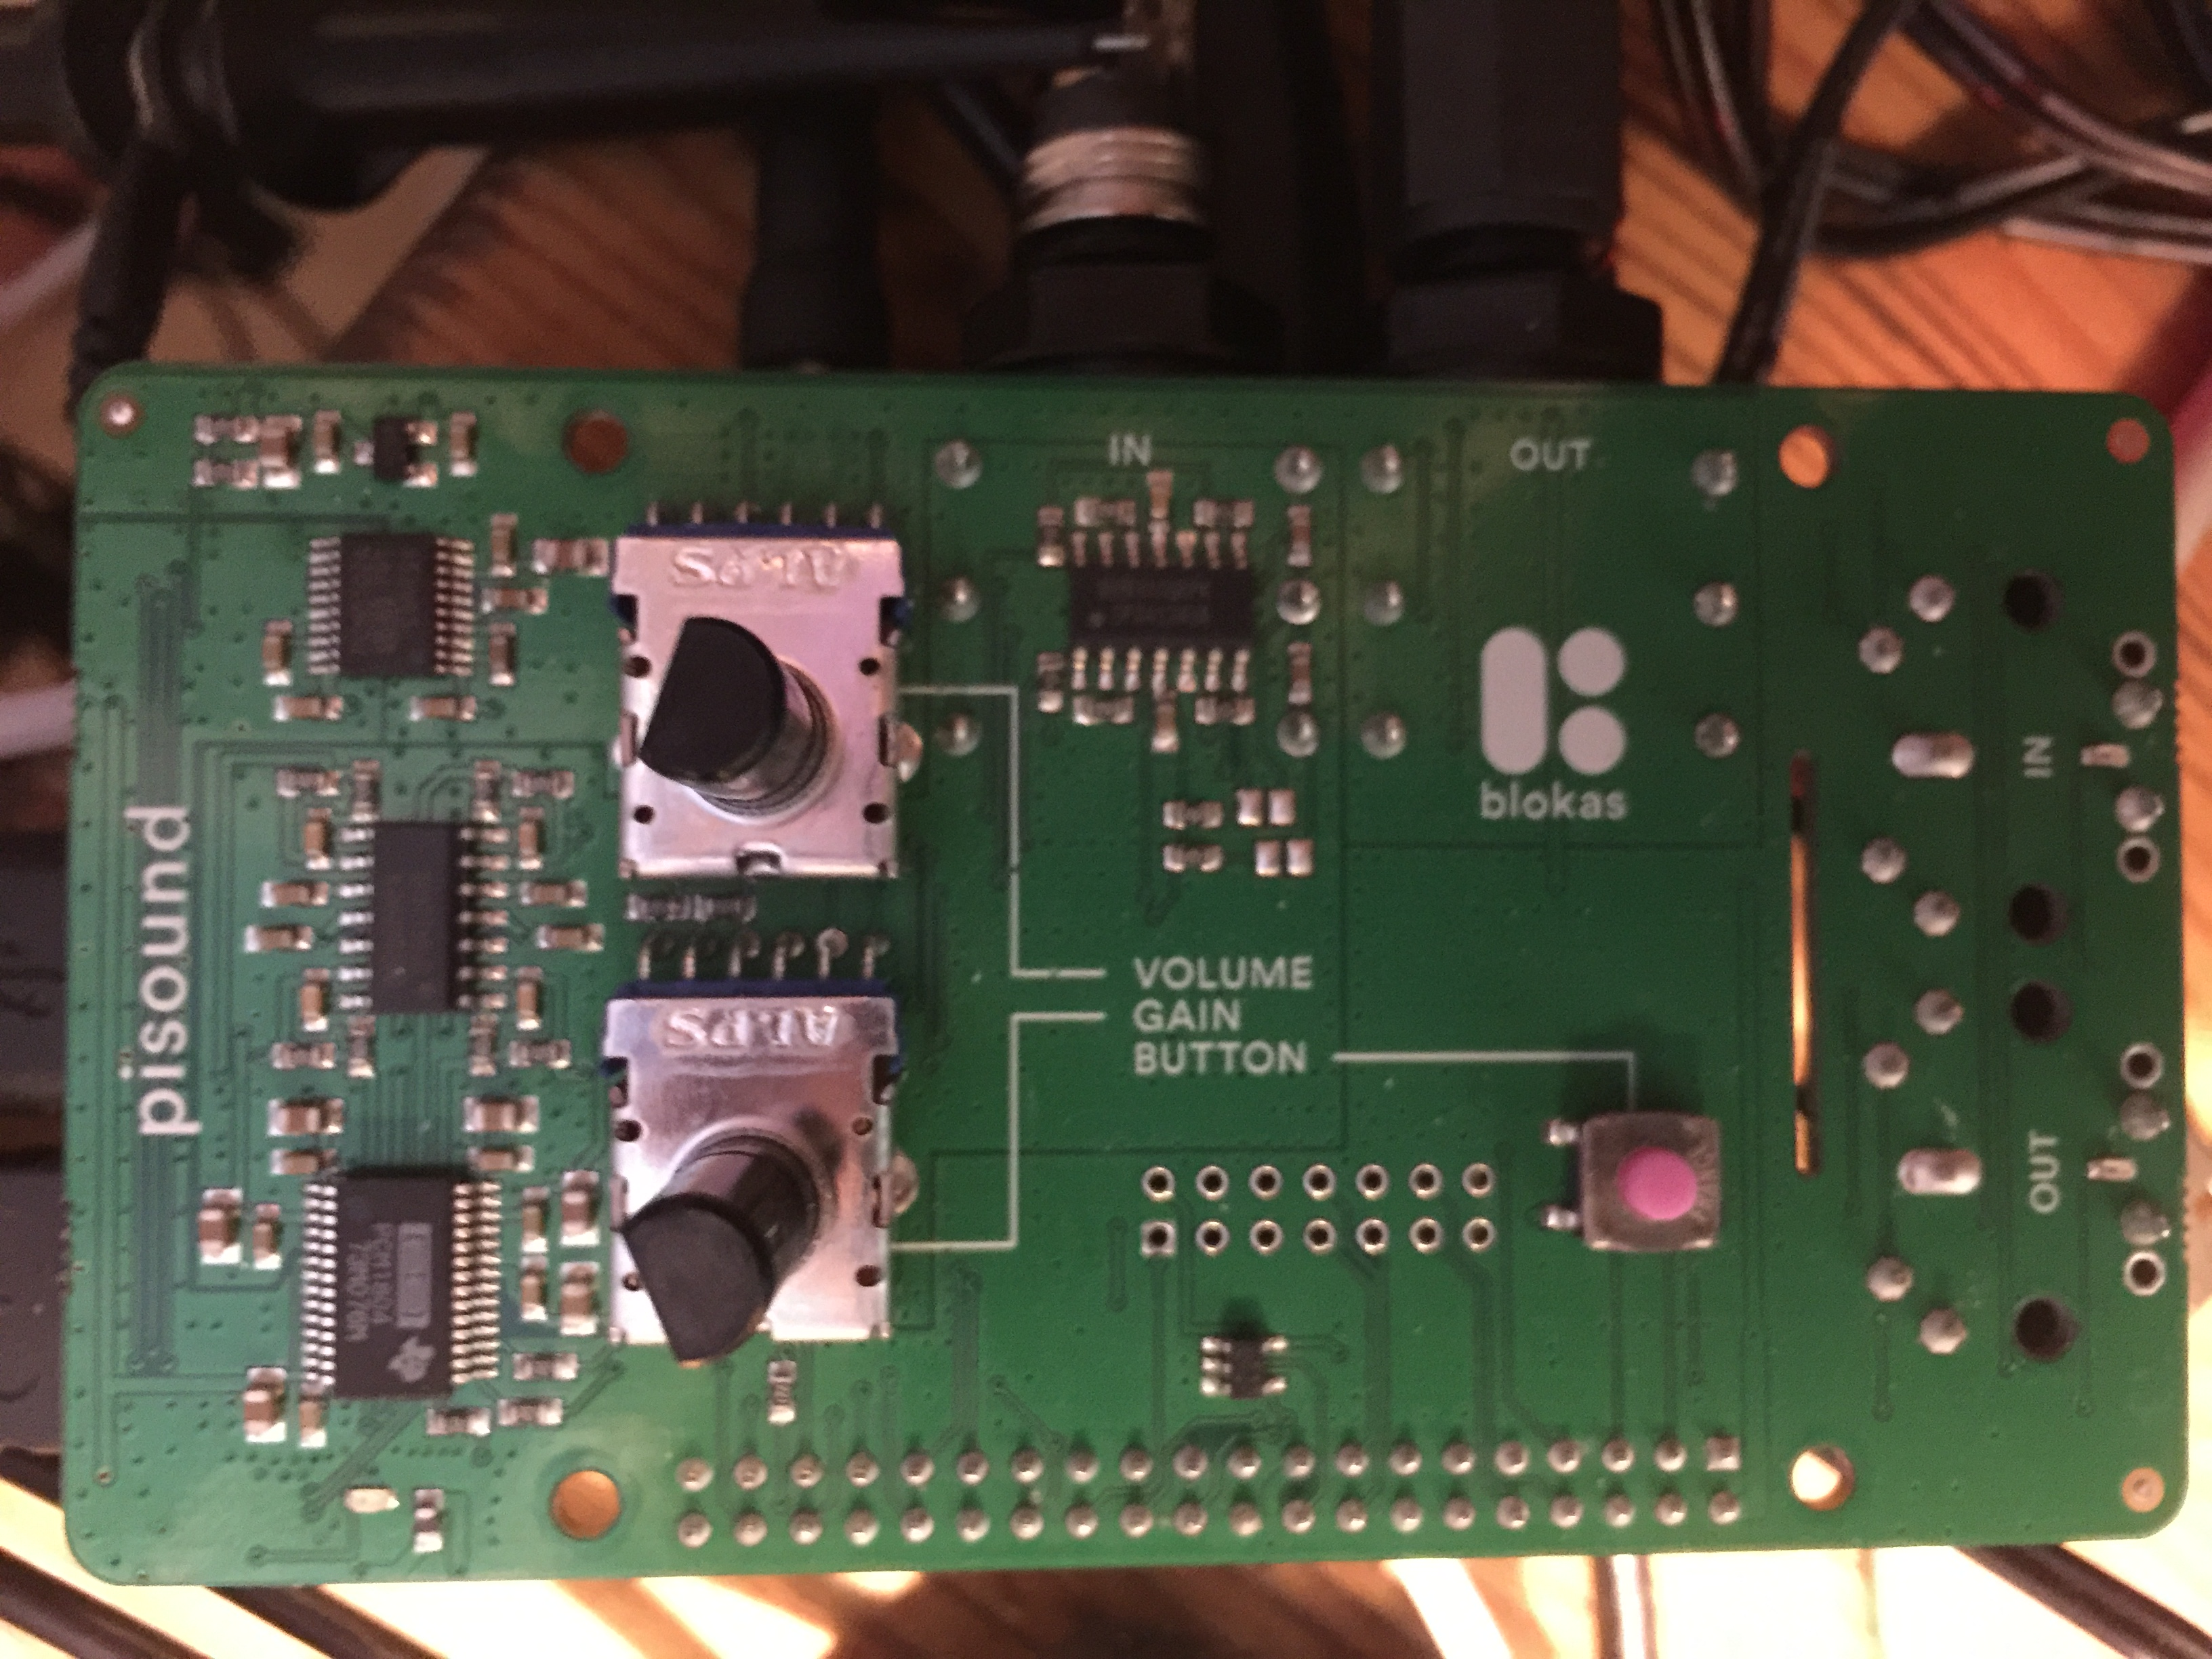
\includegraphics[scale=1.0]{Pisound.jpg}}} % Image background
\AddToShipoutPicture*{\put(45,50){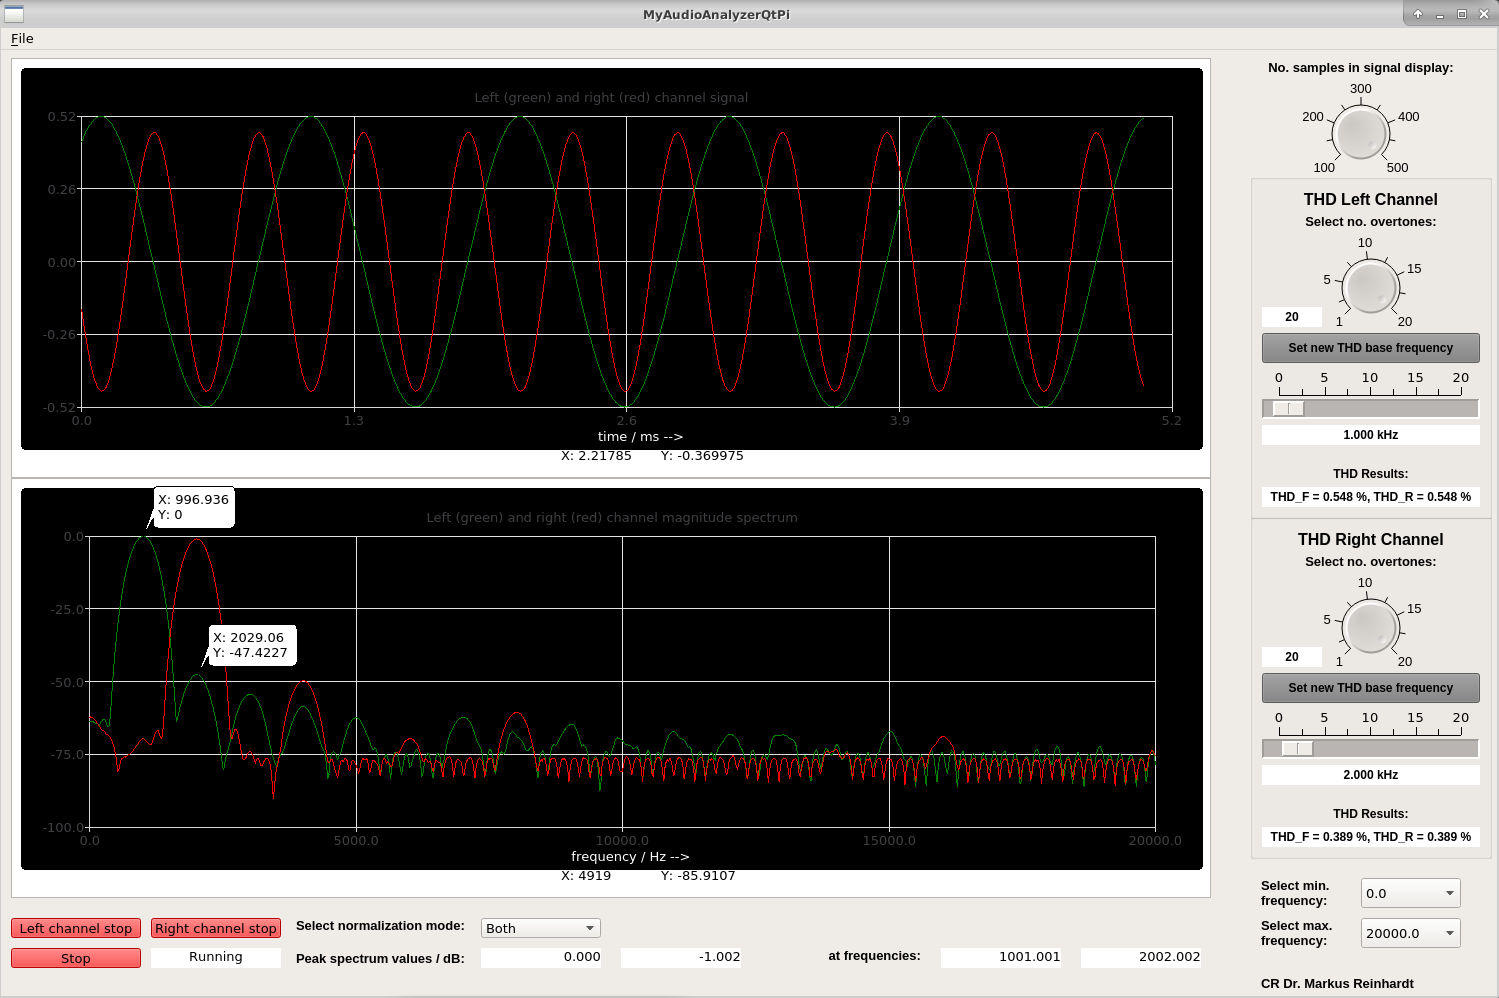
\includegraphics[scale=0.33]{MyAudioSpectrumAnalyzerGUI.png}}} % Image background

\par\normalfont\fontsize{30}{30}\sffamily\selectfont
\vspace*{-0.5cm}
{\color{black}
	\textbf{\Huge Audio Spectrum Analyzer\\ for the Raspberry Pi with Pisound board \\
		    realized in C++ with Qt/Qwt libraries}\\
	\vspace*{1.5cm}
	{\textbf\huge Documentation and User Guide}\par % Book title
	\vspace*{0.5cm}
	{\textbf \huge by Dr. Markus Reinhardt}\par % Author name
	\vspace*{1.5cm}
	{\textbf \huge \today}\par
}
\endgroup
\vfill

% \maketitle

\newpage
\thispagestyle{empty}
\tableofcontents

\thispagestyle{empty}
\listoffigures
% \listoftables

\newpage
\pagestyle{scrheadings}

\section{Overall Concept Overview}
The block diagram of the Pisound (a Raspberry Pi sound card) based spectrum analyzer is shown in figure \ref{fig:toplevelfunctionalblock}:
\begin{figure}[tbph]
	\centering
	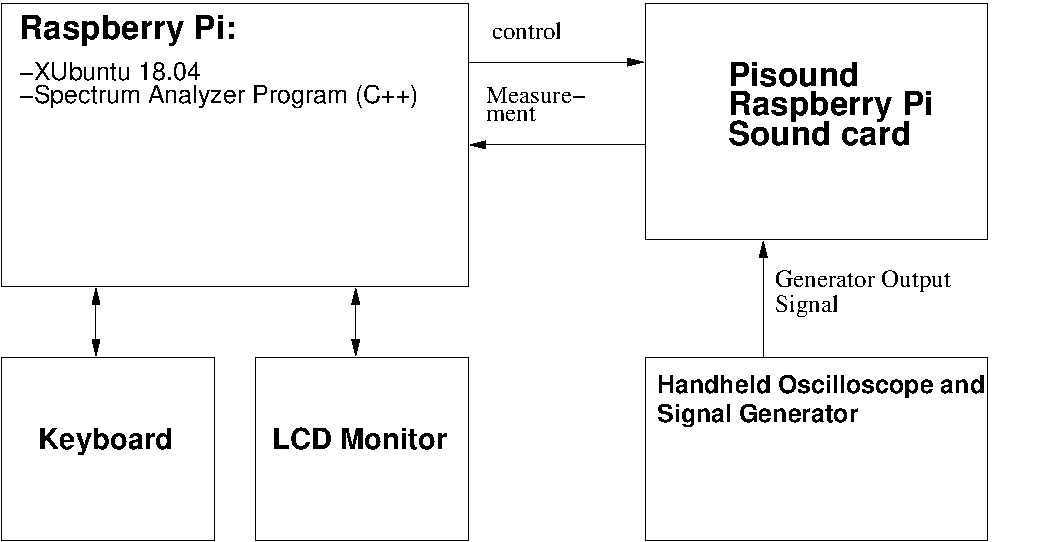
\includegraphics[width=\linewidth]{TopLevelFunctionalBlock}
	\caption[Spectrum analyzer top level block diagram]{Spectrum analyzer top level block diagram}
	\label{fig:toplevelfunctionalblock}
\end{figure}
\newpage
\section{Hardware Description}
\subsection{Pisound Board}
Figure \ref{fig:PisoundBoard} shows the top view of the Pisound board mounted on the Raspberry Pi.
\begin{figure}[tbph]
	\centering
	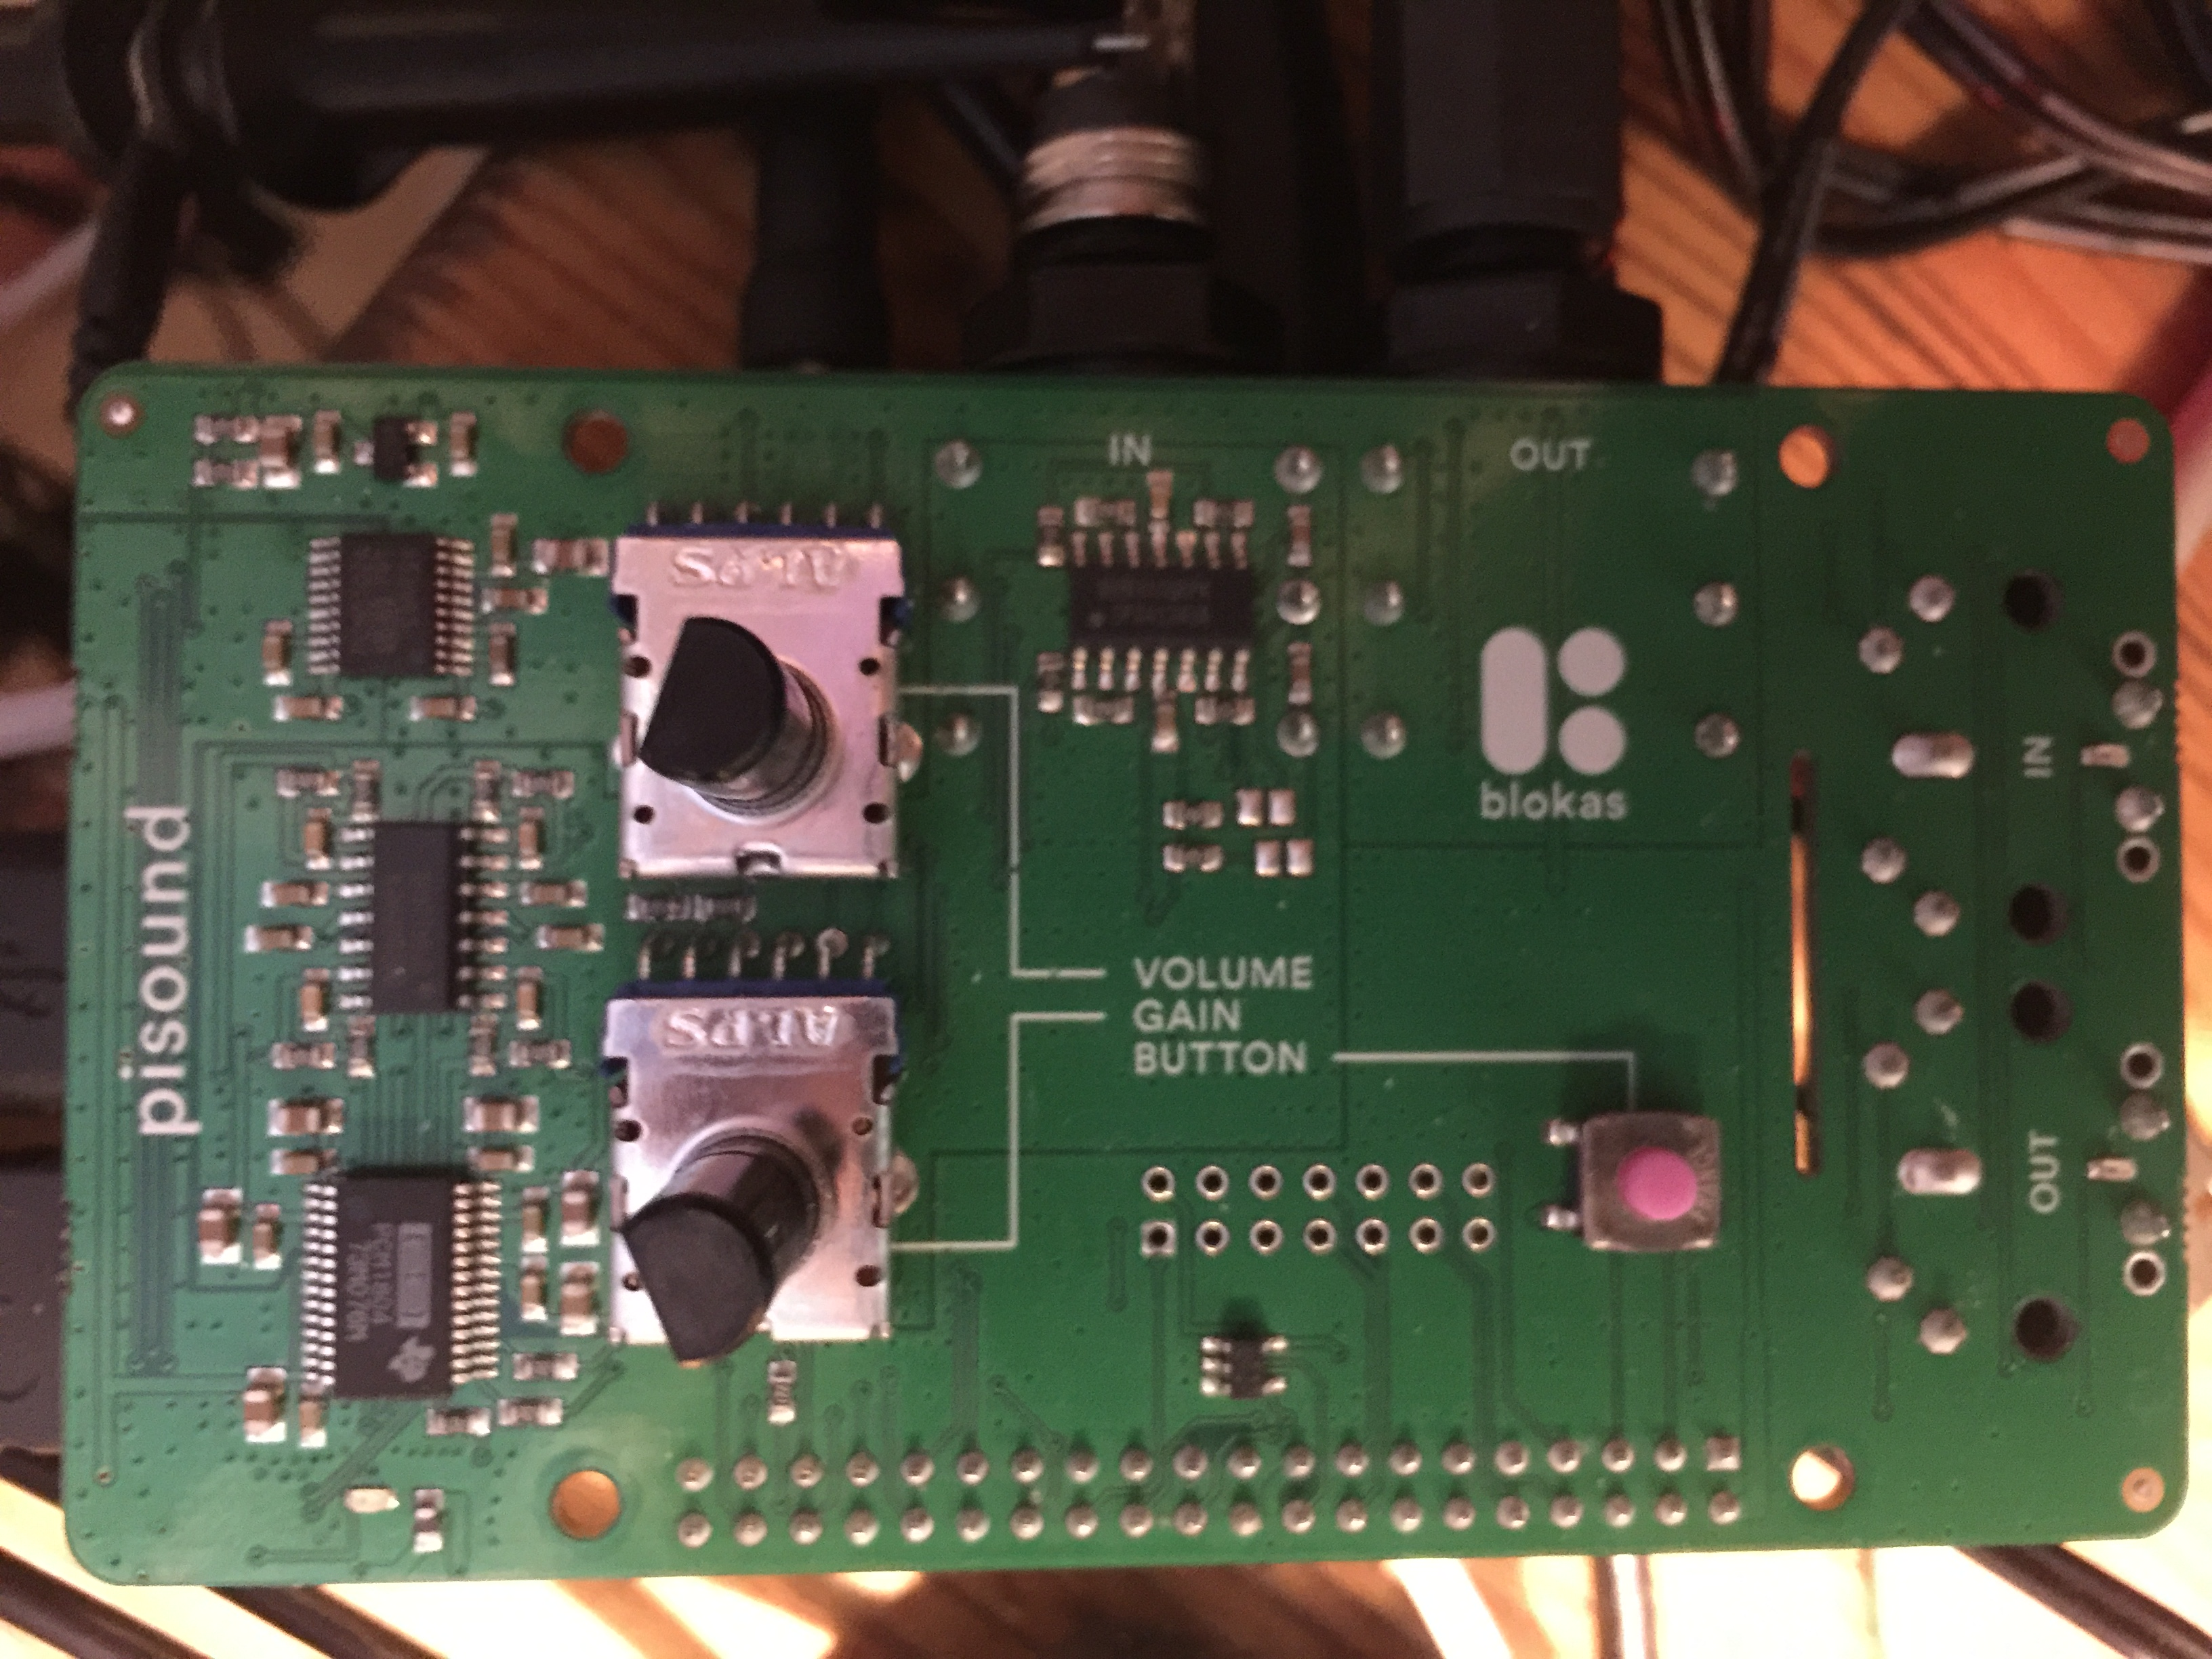
\includegraphics[width=0.9\linewidth]{Pisound.jpg}
	\caption[Pisound board]{Pisound board (top view)}
	\label{fig:PisoundBoard}
\end{figure}

The Pisound board has a PCM1804 full differential analog input 24-BIT, 192-kHz stereo A/D converter and 
a PCM5102 112dB Audio Stereo DAC with 32-bit, 384kHz PCM interface. The ADC input is fed from a OPA2134 OpAmp. 
The output of the DAC is also buffered by a OPA2134 OpAmp.
The stereo input and output signals are fed to the board via ¼" (6.35mm) sockets.

The input amplitude can be controlled by a potentiometer as well as the output volume. Both potentiometers are shown
on figure \ref{fig:PisoundBoard}.

\subsection{Casing}
The audio spectrum analyzer is housed in an aluminium case.

\newpage
\section{Software Description}
\subsection{Analyzer GUI}
Figure \ref{fig:SpectrumAnalyzerGUI} shows the GUI for the audio spectrum analyzer that is realized as a C++  program using the Qt/Qwt libraries. In this case both channels are activated.
\begin{figure}[tbph]
	\centering
	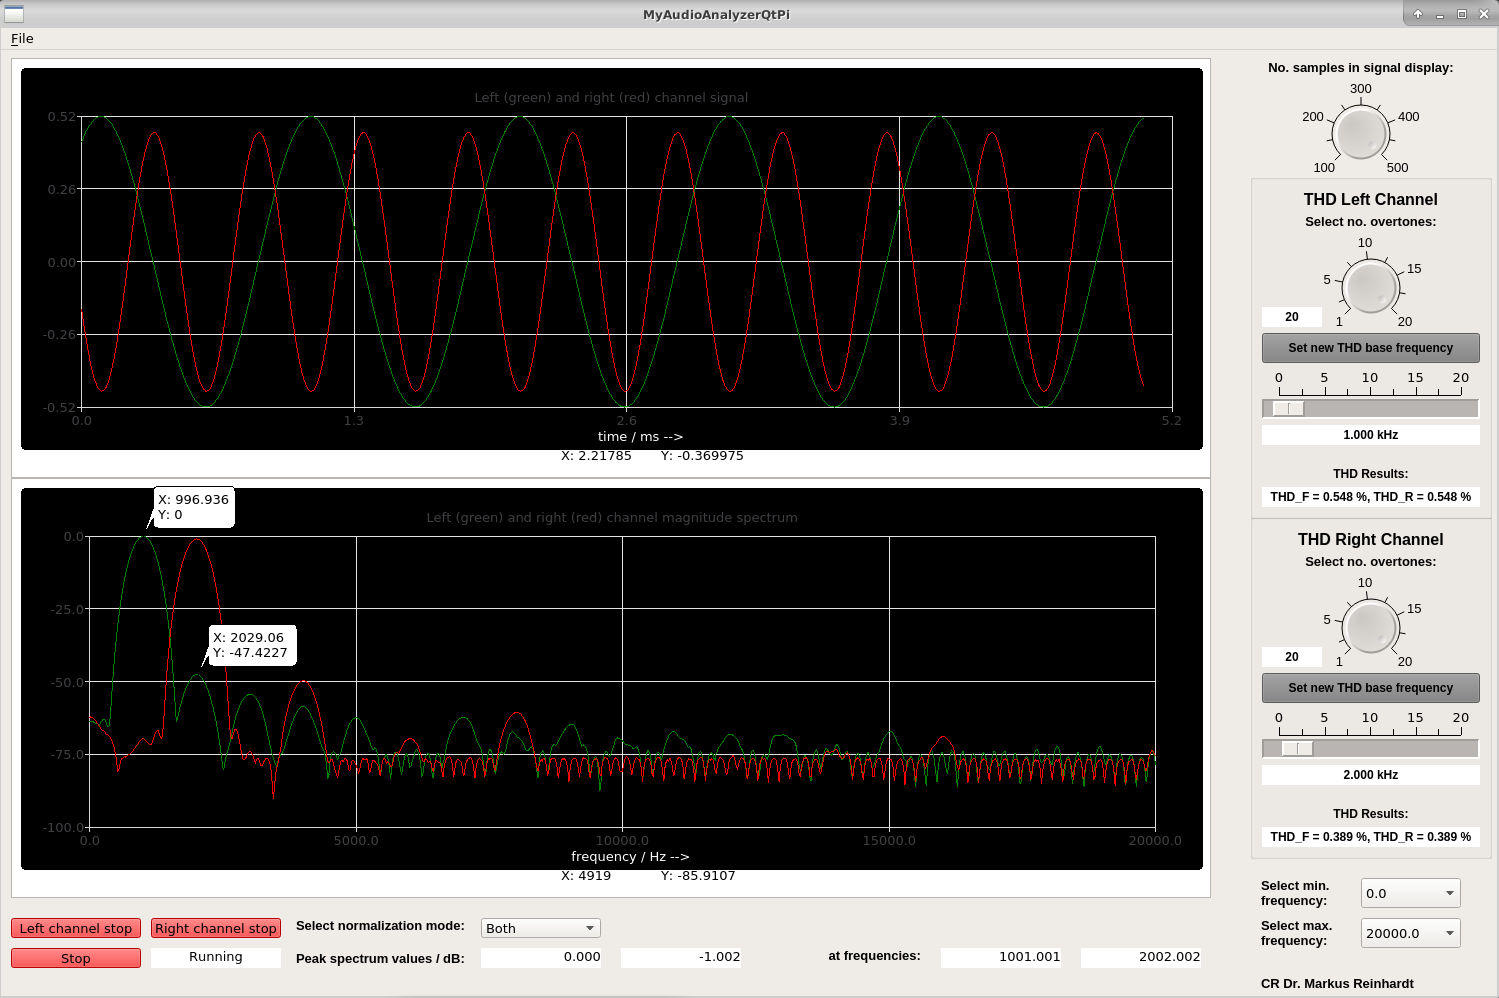
\includegraphics[width=\linewidth]{MyAudioSpectrumAnalyzerGUI.png}
	\caption[Spectrum analyzer GUI (both channels)]{Spectrum analyzer GUI (both channels)}
	\label{fig:SpectrumAnalyzerGUI}
\end{figure}

The upper left part of the GUI shows the sampled signals for the left and right channel. A dial right to the signal display allows to change the no. of samples shown in the signal display.\\
The lower left part shows the corresponding calculated spectra of the left and right channel. In the lower right corner of the GUI there are two combo boxex that allow to change the upper and lower frequency range limits of the spectrum display.\\
In the middle of the right part of the GUI the control and display for the calculation of the THD of the left and right channel are shown. For each channel the number of overtones used in THD calculations are controlled by a knob and a related display. The base frequency of THD calculations can be controlled with a slider and the related display of the base frequency. The continuously calculated $THD_F$ and $THD_R$ values are shown below the controls. \\
The lower part of the GUI shows the control buttons and measurements.\\

The program is started with the command MyAudioAnalyzerQtPi.\\

The start/stop-button labeled either "Start" or "Stop" (depending on the processing status) at the left bottom corner of the GUI is used to start or stop the signal capturing, the spectrum calculations and the display of signals and spectra.
When the analyzer is stopped the button's background color is green and the label is "Start". When the analyzer is running the button's background color is red and the label is "Stop".\\

The label next to the start/stop-button displayes the status, either "Running" or "Stopped".
 
Hitting the button "Stop" will stop the spectrum calculation process.\\

With the buttons "Left Channel On/Off" or "Right Channel On/Off" the processing and display of the relevant channel(s) is activated or deactivated.\\

With the selector right to the text "Select normalization mode" the mode how to do the normalization of the
calculated signal spectra can be chosen. There are four modes:
\begin{itemize}
	\item "Both": Both spectra are normalized with the maximum magnitude value determined of both channels.
	\item "Left": Both spectra are normalized with the maximum magnitude value of the left channel.
	\item "Right": Both spectra are normalized with the maximum magnitude value of the right channel.
	\item "Separate": Each spectrum is normalized with the maximum magnitude value of the corresponding channel separately.
\end{itemize}

With "Ctrl-Q" the program is quit. \\

With "Ctrl-S" the signals and spectra are saved (in file SignalAndSpectra.csv).\\

Also the peak values of the calculated spectra (in dB) and the corresponding location in frequency domain of the peaks are displayed on the status line for both channels (if they are activated).\\

Figure \ref{fig:SpectrumAnalyzerGUI2} shows the GUI for the audio spectrum analyzer in the case that only the left channel is activated.
\begin{figure}[tbph]
	\centering
	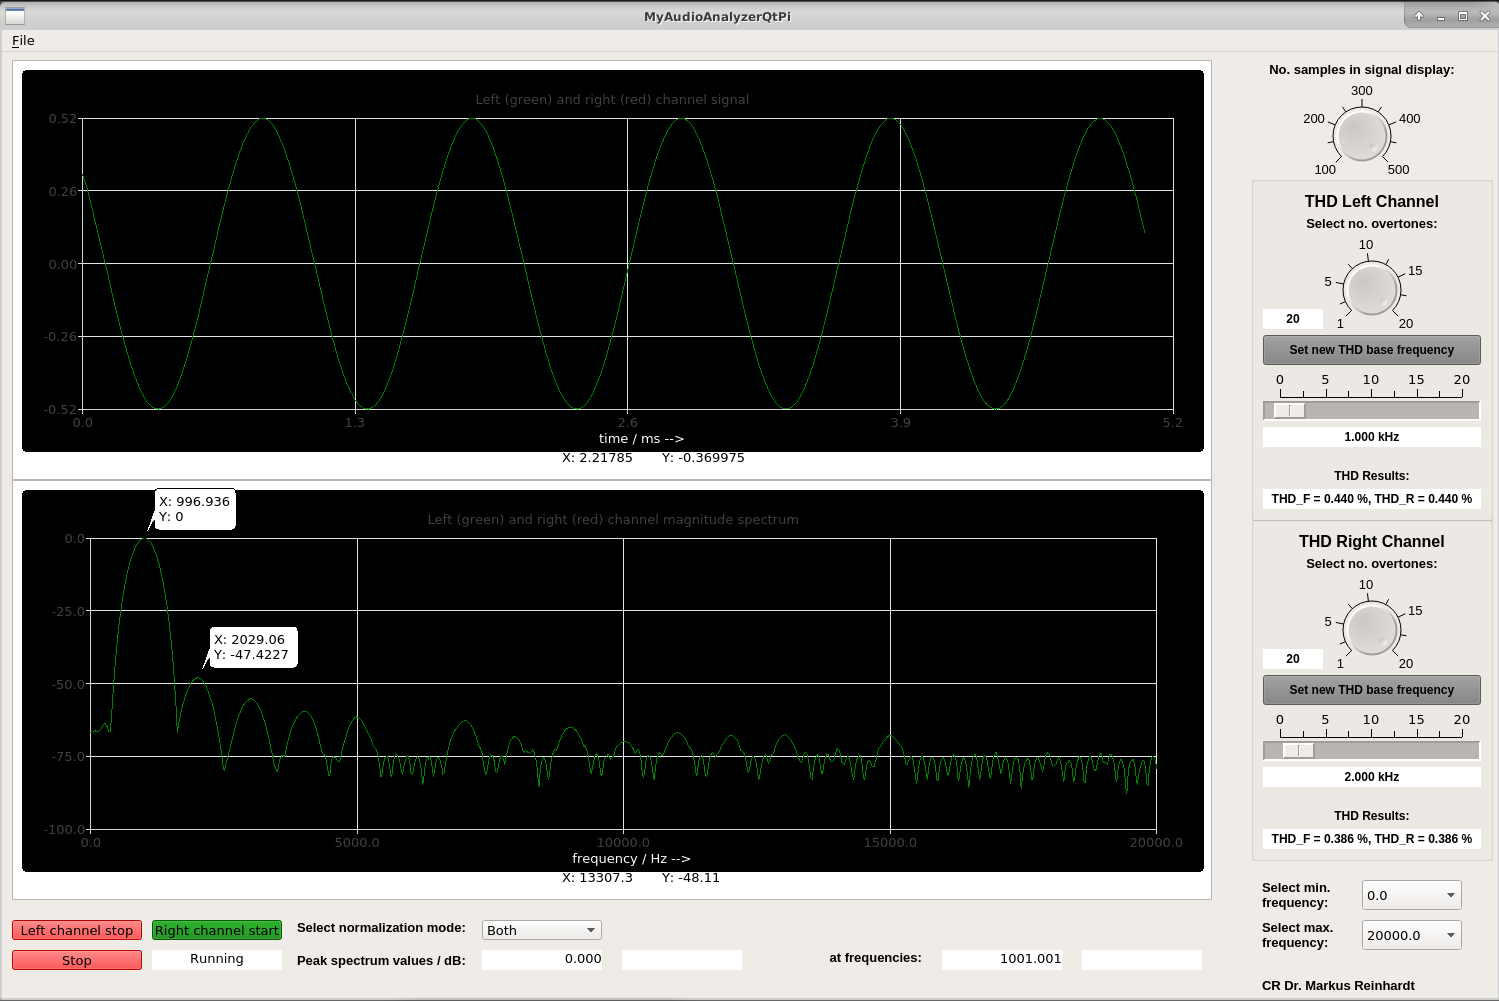
\includegraphics[width=\linewidth]{MyAudioSpectrumAnalyzerGUILeftChannel.png}
	\caption[Spectrum analyzer GUI (single channel)]{Spectrum analyzer GUI (single channel)}
	\label{fig:SpectrumAnalyzerGUI2}
\end{figure}

\subsection{Postprocessing Tools}
A python script (TestLoadSpectrumDataCSV.py) can be used to load and display the stored signals and spectra from file SignalAndSpectra.csv.
Figure \ref{fig:TestLoadSpectraCSVDisplays} shows the figures that are created by the program based on the stored spectra generated by the audio spectrum analyzer.
\begin{figure}[tbph]
	\centering
	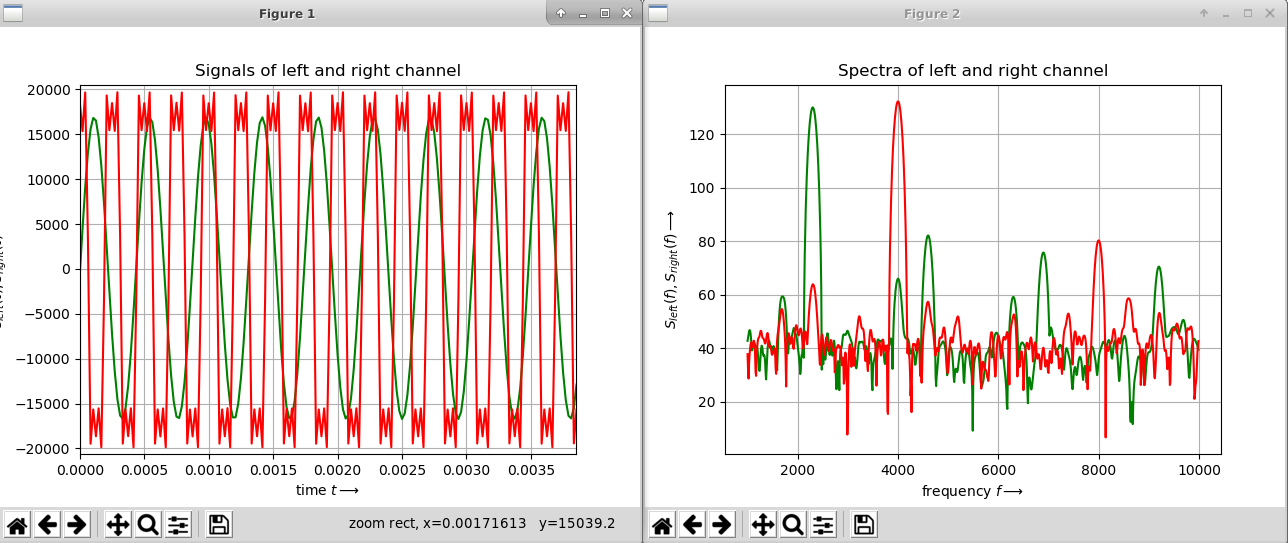
\includegraphics[width=\linewidth]{TestLoadSpectraCSVDisplays.png}
	\caption[Figures of loaded and postprocessed signals and spectra]{Figures of loaded and postprocessed signals and spectra}
	\label{fig:TestLoadSpectraCSVDisplays}
\end{figure}

\appendix{\textbf{ToDo}}
\begin{itemize}
	\item Convert to thread based processing, MMI thread with higher priority, DTFT processing with lower priority
\end{itemize}


\end{document}  